\documentclass[lettersize,journal]{IEEEtran}
\usepackage{amsmath,amsfonts,amssymb}
\usepackage{algorithmic}
\usepackage{algorithm}
\usepackage{array}
\usepackage{booktabs}
\usepackage[caption=false,font=normalsize,labelfont=sf,textfont=sf]{subfig}
\usepackage{textcomp}
\usepackage{stfloats}
\usepackage{orcidlink}
\usepackage{url}
\usepackage{graphicx}
\usepackage{cite}
\usepackage{xcolor}
\usepackage{multirow}
\usepackage{makecell}
\usepackage{tikz}
\usetikzlibrary{positioning,fit,arrows.meta,backgrounds,calc}
\usepackage{hyperref}
\hypersetup{colorlinks=true,linkcolor=blue,citecolor=blue,urlcolor=blue}

% Notation shortcuts
\newcommand{\tmfl}{\textsc{TrustMesh-FL}}
\newcommand{\tm}{\textsc{TrustMesh}}
\newcommand{\ie}{\textit{i.e.}}
\newcommand{\eg}{\textit{e.g.}}

% Figure placeholder command
\newcommand{\figplaceholder}[2]{%
    \begin{center}
    \fbox{\parbox{0.9\columnwidth}{\centering\vspace{#1}\textsc{[Figure Placeholder]}\\[4pt]\small #2\vspace{#1}}}
    \end{center}
}

\hyphenation{op-tical net-works semi-conduc-tor IEEE-Xplore}

\begin{document}

\title{TrustMesh-FL: Consensus-Validated Federated Learning for Trustless Heterogeneous IoT Environments}

\author{Murtaza~Rangwala\orcidlink{0009-0003-4578-8671},~\IEEEmembership{Member,~IEEE,}
        Richard~O.~Sinnott\orcidlink{0000-0001-5998-222X},~\IEEEmembership{}
        and~Rajkumar~Buyya\orcidlink{0000-0001-9754-6496},~\IEEEmembership{Fellow,~IEEE}
\\
\IEEEcompsocitemizethanks{
  \IEEEcompsocthanksitem Murtaza Rangwala, Richard O. Sinnott and Rajkumar Buyya are with the Quantum Cloud Computing and Distributed Systems (qCLOUDS) Lab, School of Computing and Information Systems, The University of Melbourne, Australia.
}
}

\maketitle

% ============================================================================
\begin{abstract}
Federated learning (FL) enables distributed model training across heterogeneous IoT nodes without centralising raw data, yet its correctness guarantee rests entirely on an honest aggregation server, an assumption that cannot be enforced in open, trustless environments where compute infrastructure is unverified. Existing blockchain-integrated FL systems address auditability by recording model hashes or metadata on-chain, but the aggregation computation itself remains off-chain and unchecked, leaving a fundamental trust gap. This paper presents \tmfl{}, an extension of the \tm{} blockchain-enabled distributed computing framework in which federated aggregation is elevated to a first-class blockchain transaction. Every Practical Byzantine Fault Tolerance (PBFT) validator independently re-executes the FedAvg computation and validates the resulting model against a shared test dataset before the aggregated weights are accepted into blockchain state. A malicious or faulty aggregator is therefore detected and rejected through consensus before its output propagates to participating nodes. \tmfl{} is evaluated on a physical K3s cluster across multiple federated rounds under varying non-IID data distributions (Dirichlet $\alpha \in \{0.1, 0.5, 1.0, 10.0\}$), Byzantine attack scenarios, and network scales of up to ten IoT nodes. Results demonstrate that consensus-validated aggregation introduces \textcolor{red}{[X\%]} overhead relative to a non-validated baseline, that all three tested Byzantine attack classes are detected and rejected with \textcolor{red}{[Y\%]} accuracy, and that round completion time scales sub-linearly with the number of participating nodes.
\end{abstract}

\begin{IEEEkeywords}
Federated Learning, Internet of Things, Blockchain, Byzantine Fault Tolerance,
Distributed Systems, Hyperledger Sawtooth, PBFT, Trustless Computing, Edge Computing
\end{IEEEkeywords}

% ============================================================================
\section{Introduction}
\label{sec:intro}
% ============================================================================

\IEEEPARstart{T}{he} proliferation of Internet of Things (IoT) devices has produced
distributed data generation at a scale that renders centralised processing increasingly
impractical. Federated learning (FL)~\cite{mcmahan2017communication} has emerged as a
principal paradigm for training machine learning models across these devices without
transmitting raw data, preserving privacy while exploiting local computational capacity.
Standard FL protocols, however, rest on a critical trust assumption: the aggregation server
must faithfully compute and return the federated average of client updates. In open,
heterogeneous IoT deployments where compute nodes may be owned and operated by distinct,
mutually distrusting parties, this assumption cannot be enforced by protocol design alone.

The consequences of a compromised aggregator are substantial. A malicious aggregator may
inject arbitrary weights into the global model, selectively exclude contributions, or
subtly bias the federated average in ways that are undetectable to individual clients.
Unlike Byzantine attacks on IoT nodes themselves, which have received considerable attention
through robust aggregation rules such as Krum~\cite{blanchard2017machine}, Trimmed
Mean~\cite{yin2018byzantine}, and Bulyan~\cite{elMhamdi2018hidden}, the threat of a
dishonest aggregator is structural: it arises after all honest nodes have submitted their
updates, and before any of them receive the result. Robust aggregation rules address the
former problem; they do not address the latter.

Blockchain technology has been proposed as a mechanism for establishing trust in FL
pipelines. BlockFL~\cite{kim2020blockchained} logs local model updates on-chain;
FedChain~\cite{li2021fedchain}, BFLC~\cite{bflc2020}, and
DeepChain~\cite{weng2021deepchain} record gradient metadata and participation proofs to
support incentive mechanisms and post-hoc auditing. These approaches improve accountability,
but they are fundamentally reactive: the blockchain provides an immutable record of what
was \emph{submitted}, not a verification of what was \emph{computed}. Aggregation remains
the responsibility of a single designated entity, and the trust problem is displaced rather
than resolved.

This paper proposes a different architectural approach. In \tmfl{}, model aggregation is
not delegated to a trusted party and audited after the fact; it is executed as a blockchain
transaction and verified by every PBFT validator before the result is committed to state.
The system extends \tm{}~\cite{rangwala2025trustmesh}, a framework providing Byzantine
fault-tolerant task scheduling for heterogeneous IoT environments over Hyperledger Sawtooth,
with two new transaction processors and a two-phase FL protocol. The core mechanism is as
follows: when an aggregator compute node submits an aggregation confirmation transaction,
the confirmation transaction processor running on every PBFT validator independently
fetches the same model weights from a distributed CouchDB store, re-executes the
sample-weighted FedAvg computation, verifies that the aggregator's result matches to within
a numerical tolerance of $10^{-6}$, and evaluates the resulting model against a shared
validation dataset. The aggregated global model is accepted into blockchain state only if
all four validation checks pass and PBFT consensus is reached. No single node, including
the designated aggregator, can commit a tampered or invalid model. A concise overview of
the \tm{} base framework on which \tmfl{} builds is provided in
Section~\ref{sec:preliminaries}.

This design choice carries a quantifiable cost. Moving verification inside consensus
introduces per-round overhead proportional to the model size and the number of validators.
A central empirical contribution of this work is the measurement of that cost in a
representative physical deployment, and the characterisation of conditions under which
it is warranted.

The novel contributions of this paper, beyond those of the prior \tm{}
publication~\cite{rangwala2025trustmesh}, are as follows:

\begin{enumerate}

    \item \textbf{Consensus-validated aggregation:} A protocol in which FedAvg is
    independently re-computed by every PBFT validator, ensuring that a compromised
    aggregator cannot propagate manipulated weights without detection. This constitutes
    a new architectural principle: aggregation \emph{correctness} as a consensus
    property rather than a trust assumption.

    \item \textbf{Two-phase FL protocol:} A federated learning protocol that integrates
    with the existing \tm{} workflow scheduling and task execution pipeline. Phase~1
    dispatches local training through the standard \tm{} IoT data and scheduling pipeline;
    Phase~2 introduces time-windowed weight collection and blockchain-consensus aggregation.
    Non-FL workloads are unaffected.

    \item \textbf{Model validation pipeline:} A four-stage deterministic validation
    procedure executed inside the confirmation transaction processor, covering weight
    magnitude, weight distribution, model sanity, and accuracy against a shared validation
    dataset, providing defence-in-depth against both Byzantine attacks and aggregator
    misconfiguration.

    \item \textbf{Empirical overhead characterisation:} A quantitative evaluation of the
    latency cost of consensus-validated aggregation relative to a non-validated baseline,
    across four non-IID data regimes ($\alpha \in \{0.1, 0.5, 1.0, 10.0\}$), three
    Byzantine attack classes, and IoT network scales from four to ten nodes on a physical
    K3s cluster.

\end{enumerate}

Experimental results show that \tmfl{} converges under moderate non-IID conditions
($\alpha = 0.5$) within \textcolor{red}{[Z]} rounds on MNIST, that consensus validation
introduces \textcolor{red}{[X\%]} additional per-round latency over a passthrough baseline,
that all three Byzantine attack classes (random noise injection, sign flipping, and weight
scaling) are detected and rejected with \textcolor{red}{[Y\%]} accuracy, and that round
completion time grows sub-linearly as the number of participating IoT nodes scales from
four to ten.

The remainder of this paper is organised as follows.
Section~\ref{sec:related} surveys related work in federated learning, Byzantine-robust
aggregation, and blockchain-integrated FL.
Section~\ref{sec:preliminaries} provides a brief overview of the \tm{} base framework
as prerequisite context for the design described in this paper.
Section~\ref{sec:design} presents the \tmfl{} system architecture and two-phase protocol.
Section~\ref{sec:implementation} describes the implementation.
Section~\ref{sec:evaluation} presents the experimental evaluation and results.
Section~\ref{sec:discussion} examines trade-offs and limitations.
Section~\ref{sec:conclusion} concludes and outlines future work.

% ============================================================================
\section{Related Work}
\label{sec:related}
% ============================================================================

\subsection{Federated Learning}

McMahan et al.~\cite{mcmahan2017communication} introduced FedAvg, establishing the
canonical federated learning protocol in which clients perform multiple local gradient
descent steps before transmitting model updates to a central aggregator. Subsequent work
identified data heterogeneity as a primary challenge: when client data distributions diverge
significantly, local updates may conflict and slow global convergence~\cite{zhao2018federated}.
FedProx~\cite{li2020federated} addressed this by introducing a proximal regularisation term
that constrains local updates to remain close to the current global model, improving
convergence stability under non-IID conditions. Communication efficiency has also received
significant attention, with structured and compressed update schemes reducing the bandwidth
cost of client-to-server transmission~\cite{konecny2016federated}.

A shared assumption across these works is that the aggregation server is trusted: it
receives client updates, applies the specified aggregation rule faithfully, and returns a
correct global model. In open IoT environments where compute infrastructure is heterogeneous
and untrusted, this assumption requires explicit enforcement by the protocol.

\subsection{Byzantine-Resilient Federated Learning}

Byzantine-resilient aggregation rules defend against clients that submit corrupted or
adversarially crafted updates. Krum~\cite{blanchard2017machine} selects the client update
with the smallest sum of squared distances to its neighbours, isolating outliers.
Trimmed Mean~\cite{yin2018byzantine} applies coordinate-wise trimmed averaging, discarding
the most extreme values in each parameter dimension. Bulyan~\cite{elMhamdi2018hidden}
combines multi-Krum selection with trimmed mean aggregation to improve robustness against
adaptive attacks. FLTrust~\cite{cao2020fltrust} uses a small server-side clean dataset to
score client updates, accepting only those whose gradient direction aligns with the server's
own gradient.

These methods address Byzantine behaviour at the client level. They presuppose that the
entity applying the aggregation rule is itself honest. If the aggregator is compromised, it
may selectively apply or ignore any of these rules, apply them to a manipulated subset of
updates, or return an output that was not computed from the submitted gradients at all.
\tmfl{} is orthogonal to Byzantine-resilient aggregation rules: the validation pipeline
currently uses standard FedAvg, but the consensus-validated architecture is rule-agnostic
and could accommodate Krum or Trimmed Mean as a drop-in replacement for the aggregation
step while preserving the correctness guarantee.

\subsection{Blockchain-Integrated Federated Learning}

BlockFL~\cite{kim2020blockchained} records local model updates on-chain, enabling
contribution provenance tracking and supporting a cryptocurrency-based incentive mechanism.
However, the aggregation itself is performed off-chain by a central coordinator; the
blockchain records what was submitted, not the correctness of the aggregated result.

FedChain~\cite{li2021fedchain} and BFLC~\cite{bflc2020} use blockchain primarily for
incentive distribution and participation accounting. Both frameworks maintain a designated
aggregation server that processes updates off-chain, with the blockchain serving as an
auditable ledger of contributions and rewards.

DeepChain~\cite{weng2021deepchain} stores gradient commitments on-chain and introduces a
chained gradient protocol to detect gradient manipulation across rounds. The aggregated
model is nonetheless produced by a single entity, and the trust problem for the aggregator
remains unaddressed.

Biscotti~\cite{shayan2021biscotti} decentralises aggregation through a peer-to-peer
protocol in which all participants evaluate each other's updates. While this eliminates the
single aggregator, it requires each client to receive and process every other client's
update, introducing communication costs that scale as $O(N^2)$ in the number of clients
and are prohibitive for IoT deployments with constrained network bandwidth.

The key distinction between all prior systems and \tmfl{} is the following: prior systems
treat the aggregation computation as a pre-consensus step that the blockchain records;
\tmfl{} treats the aggregation computation as a within-consensus operation that the
blockchain verifies. This is the first system, to the authors' knowledge, in which the
correctness of FedAvg is a property enforced by distributed consensus rather than assumed
from a trusted party.

\subsection{Distributed Computing Frameworks for Trustless IoT}

The integration of blockchain with fog and edge computing has been explored in several
frameworks. FogBus~\cite{tuli2019fogbus} introduced blockchain-based data logging for
fog computing but relied on a partially centralised control structure that limits
applicability in fully distributed environments. CoopEdge~\cite{yuan2021coopedge}
introduced a reputation-based consensus mechanism for cooperative edge computation.
BlockEdge~\cite{kumar2020blockedge} combined permissioned and permissionless blockchain
chains in a three-tier architecture but remained limited to simulation evaluation. A
systematic comparison of these frameworks against \tm{} is presented in
\cite{rangwala2025trustmesh}. None of the surveyed frameworks support federated learning
with verifiable aggregation. \tmfl{} addresses this gap by extending \tm{}'s trust
guarantees to the FL aggregation computation.

% ============================================================================
\section{The \tm{} Framework}
\label{sec:preliminaries}
% ============================================================================

\tm{}~\cite{rangwala2025trustmesh} is a blockchain-enabled distributed computing framework
for trustless, heterogeneous IoT environments, implemented over Hyperledger
Sawtooth~\cite{hyperledger2018sawtooth} with PBFT consensus. It provides the
infrastructure on which \tmfl{} builds. This section summarises the components
of \tm{} that are directly referenced in subsequent sections; full architectural details
are available in~\cite{rangwala2025trustmesh}.

\subsubsection*{Three-Layer Architecture}

\tm{} organises its components into three layers, illustrated in Fig.~\ref{fig:arch}.
The \textbf{Network Management Layer} hosts control nodes that manage application
deployment and workflow orchestration. Applications are distributed as Docker images
whose content digests are cryptographically signed and verified against entries stored
on the blockchain. Workflows are defined as directed acyclic graphs (DAGs) representing
dependencies between applications and are stored immutably in blockchain state.

The \textbf{Computation Layer} comprises compute nodes that function simultaneously as
blockchain validators and task executors. Each compute node runs a Docker-in-Docker
environment, enabling execution of arbitrary containerised workloads. Node resources
(CPU, memory) are monitored at configurable intervals, published to a Redis cluster for
immediate access by scheduling logic, and periodically committed in batches to the
blockchain for auditability.

The \textbf{Perception Layer} contains IoT nodes that submit sensor data as workflow
transactions and receive processed results. Communication between IoT nodes and the
computation layer uses ZeroMQ (ZMQ) with CURVE25519 public-key authentication.

\subsubsection*{Multi-Phase Commit Protocol for Scheduling}

A distinctive challenge in \tm{} is that standard PBFT requires deterministic transaction
execution across all validators, yet scheduling decisions benefit from non-deterministic
algorithms such as heuristics or machine learning. \tm{} resolves this through a
multi-phase commit protocol~\cite{rangwala2025trustmesh}. In the Request and Designation
Phase ($\phi_1$), a scheduling request transaction is submitted, and a designated scheduler
node is selected deterministically by all validators. In the Generation Phase ($\phi_2$),
the designated node runs any scheduling algorithm and proposes a schedule. In the
Confirmation Phase ($\phi_3$), all validators reach PBFT consensus on the proposed schedule
by evaluating it against a set of configurable validation rules; the schedule is committed
to state only if consensus is reached. This architecture is the model on which the
\tmfl{} aggregation confirmation protocol is designed.

\subsubsection*{Data Infrastructure}

Persistent task data is stored in a CouchDB cluster with multi-master replication, providing
high-availability document storage and SHA-256 content hash verification. Temporary
coordination state, including per-node resource availability, is managed in a Redis cluster
with TLS-secured connections. This infrastructure is reused directly in \tmfl{} for model
weight storage and aggregator selection. Measured framework overhead in the base system
ranges from 3.25 to 4.19 seconds across testbeds of 4 to 16 compute nodes~\cite{rangwala2025trustmesh}.

\begin{figure}[t]
    \centering
    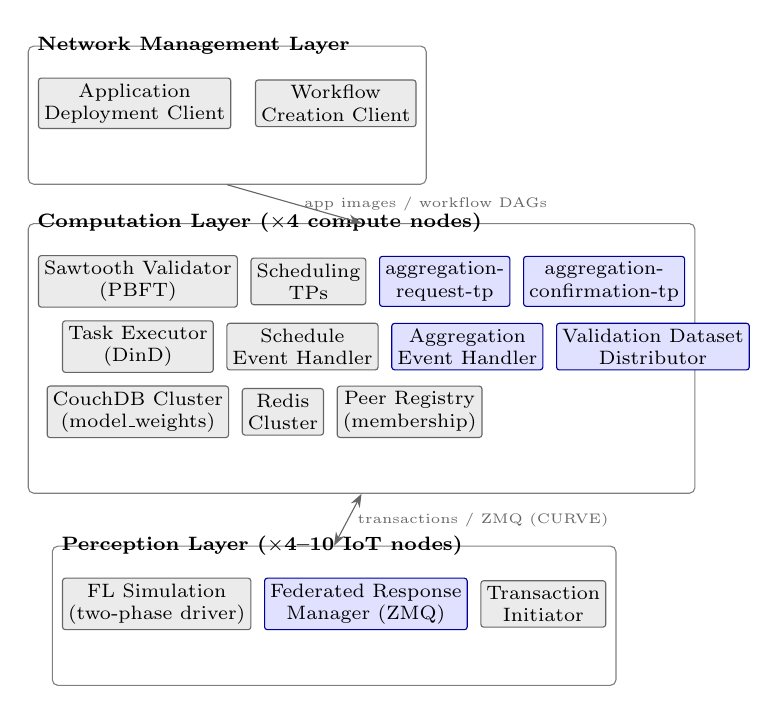
\begin{tikzpicture}[
        font=\scriptsize,
        comp/.style={draw=black!60, fill=black!8, rounded corners=1pt,
                     minimum height=4.5mm, inner sep=2pt, align=center},
        flcomp/.style={draw=blue!60!black, fill=blue!12, rounded corners=1pt,
                       minimum height=4.5mm, inner sep=2pt, align=center},
        layer/.style={draw=black!50, rounded corners=2pt, inner sep=3.5pt},
        lname/.style={font=\scriptsize\bfseries, anchor=west},
        node distance=1.6mm and 1.6mm
    ]
    % ---- Network Management Layer ----
    \node[comp] (depclient) {Application\\Deployment Client};
    \node[comp, right=3mm of depclient] (wfclient) {Workflow\\Creation Client};
    \begin{scope}[on background layer]
        \node[layer, fit=(depclient)(wfclient), label={[lname]north west:Network Management Layer},
              inner ysep=5.5mm, yshift=-1.5mm] (mgmt) {};
    \end{scope}

    % ---- Computation Layer ----
    \node[comp, below=16mm of depclient.south west, anchor=north west] (validator) {Sawtooth Validator\\(PBFT)};
    \node[comp, right=of validator] (schedtps) {Scheduling\\TPs};
    \node[flcomp, right=of schedtps] (aggreqtp) {aggregation-\\request-tp};
    \node[flcomp, right=of aggreqtp] (aggconftp) {aggregation-\\confirmation-tp};
    \node[comp, below=of validator] (taskexec) {Task Executor\\(DinD)};
    \node[comp, right=of taskexec] (schedhandler) {Schedule\\Event Handler};
    \node[flcomp, right=of schedhandler] (agghandler) {Aggregation\\Event Handler};
    \node[flcomp, right=of agghandler] (valdist) {Validation Dataset\\Distributor};
    \node[comp, below=of taskexec] (couchdb) {CouchDB Cluster\\(model\_weights)};
    \node[comp, right=of couchdb] (redis) {Redis\\Cluster};
    \node[comp, right=of redis] (peereg) {Peer Registry\\(membership)};
    \begin{scope}[on background layer]
        \node[layer, fit=(validator)(aggconftp)(couchdb)(peereg),
              label={[lname]north west:Computation Layer ($\times$4 compute nodes)},
              inner ysep=5.5mm, yshift=-1.5mm] (compl) {};
    \end{scope}

    % ---- Perception Layer ----
    \node[comp, below=26mm of taskexec.south west, anchor=north west] (simulation) {FL Simulation\\(two-phase driver)};
    \node[flcomp, right=of simulation] (fedresp) {Federated Response\\Manager (ZMQ)};
    \node[comp, right=of fedresp] (txinit) {Transaction\\Initiator};
    \begin{scope}[on background layer]
        \node[layer, fit=(simulation)(txinit),
              label={[lname]north west:Perception Layer ($\times$4--10 IoT nodes)},
              inner ysep=5.5mm, yshift=-1.5mm] (perc) {};
    \end{scope}

    % ---- Inter-layer arrows ----
    \draw[-{Stealth}, black!60] (mgmt.south) -- (compl.north)
        node[midway, right, font=\tiny] {app images / workflow DAGs};
    \draw[{Stealth}-{Stealth}, black!60] (compl.south) -- (perc.north)
        node[midway, right, font=\tiny] {transactions / ZMQ (CURVE)};
    \end{tikzpicture}
    \caption{%
        \tmfl{} system architecture. Grey components are inherited unchanged from
        \tm{}~\cite{rangwala2025trustmesh}; blue components are introduced in this work.%
    }
    \label{fig:arch}
\end{figure}

% ============================================================================
\section{System Design}
\label{sec:design}
% ============================================================================

\subsection{Design Overview}

\tmfl{} extends \tm{} with a two-phase federated learning protocol. Phase~1 (Local
Training) reuses the existing \tm{} task scheduling and execution pipeline without
modification. Phase~2 (Consensus-Validated Aggregation) introduces a new aggregation
lifecycle managed by two dedicated transaction processors:
the \texttt{aggregation-request-tp} and the \texttt{aggregation-confirmation-tp}.

The central design principle is that FedAvg aggregation is a blockchain transaction, not a
delegated computation. Every PBFT validator re-executes the aggregation and independently
validates the result; the global model is accepted into state only upon consensus. This
elevates aggregation correctness from an assumption to a verified property, closing the
trust gap identified in Section~\ref{sec:related}.

Three design decisions merit brief justification.

\textbf{Time-windowed collection over coordinator-based rounds.} An earlier design
considered electing a coordinator IoT node to manage round membership. This was rejected
in favour of a time-windowed collection period because it eliminates a single point of
failure, accommodates asynchronous IoT node availability, and simplifies the protocol
by removing the need for coordinator election at the IoT layer.

\textbf{CouchDB for model weights over blockchain state.} Storing model weights in
blockchain state would cause the Merkle tree to grow proportionally with model size per
round, quickly becoming unmanageable. Weights are instead stored in CouchDB with SHA-256
content hashes; only the document identifiers and hashes are recorded in blockchain state.
This preserves verifiability without bloating the ledger.

\textbf{Separate transaction processors over modifying existing ones.} All FL-specific
logic is encapsulated in new transaction processors and event handlers. No existing
\tm{} component is modified, ensuring that non-FL workloads are unaffected and that the
extension can be audited in isolation.

Fig.~\ref{fig:arch} illustrates the extended system architecture.
Fig.~\ref{fig:protocol} shows the two-phase protocol as a sequence diagram.

\begin{figure*}[t]
    \centering
    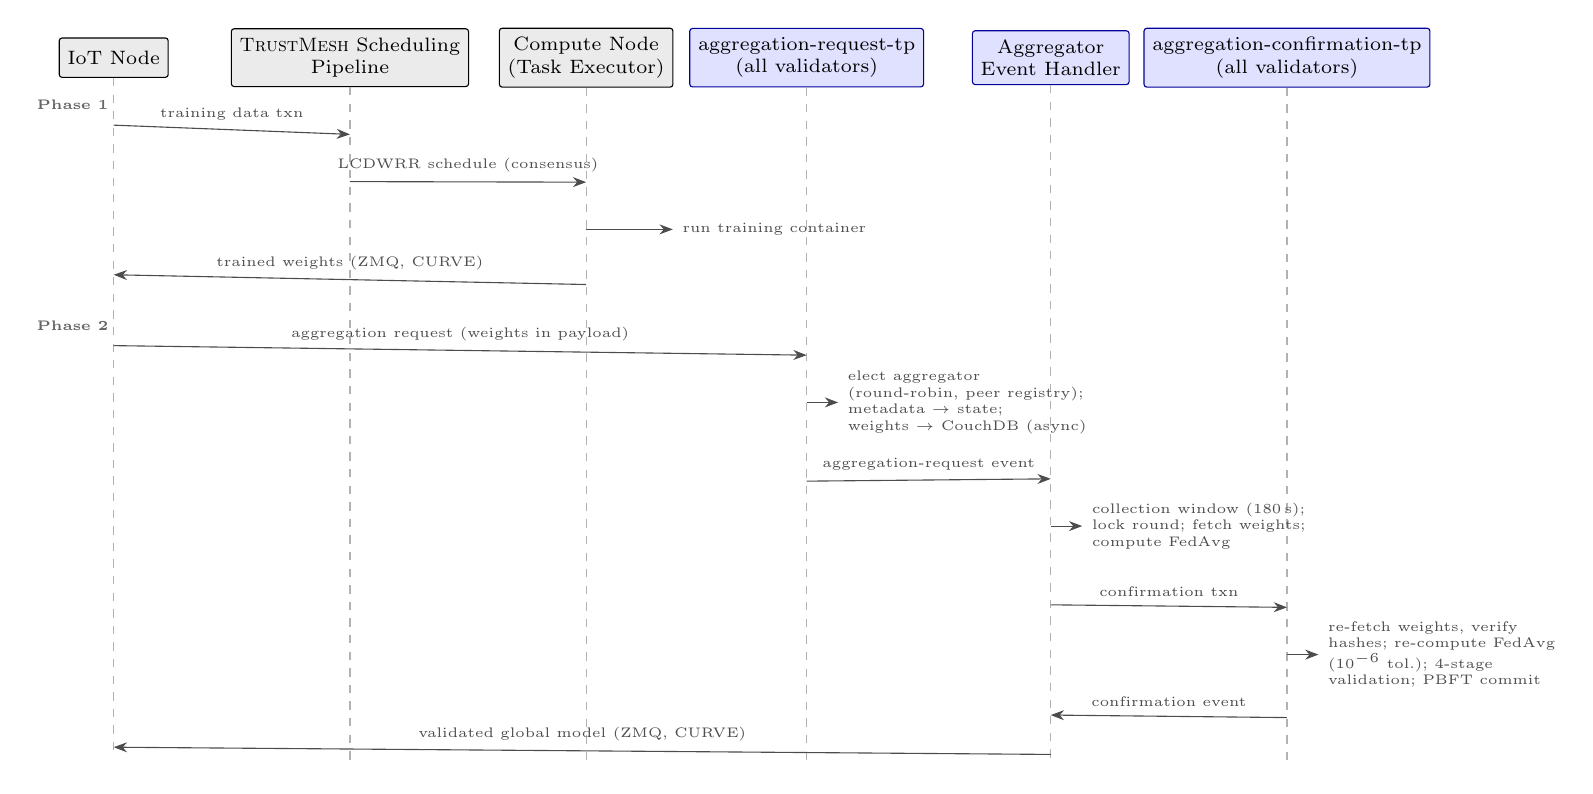
\begin{tikzpicture}[
        font=\scriptsize,
        actor/.style={draw, fill=black!8, rounded corners=1pt, minimum height=5mm,
                      inner xsep=3pt, align=center},
        flactor/.style={actor, draw=blue!60!black, fill=blue!12},
        msg/.style={-{Stealth}, black!70},
        note/.style={font=\tiny, midway, above, sloped=false},
        lifeline/.style={black!30, dashed}
    ]
    % Lifelines (x positions)
    \node[actor]   (iot)   at (0,0)    {IoT Node};
    \node[actor]   (sched) at (3.0,0)  {\tm{} Scheduling\\Pipeline};
    \node[actor]   (exec)  at (6.0,0)  {Compute Node\\(Task Executor)};
    \node[flactor] (reqtp) at (8.8,0)  {aggregation-request-tp\\(all validators)};
    \node[flactor] (aggh)  at (11.9,0) {Aggregator\\Event Handler};
    \node[flactor] (conftp)at (14.9,0) {aggregation-confirmation-tp\\(all validators)};

    \foreach \n/\len in {iot/8.6, sched/8.6, exec/8.6, reqtp/8.6, aggh/8.6, conftp/8.6}
        \draw[lifeline] (\n.south) -- ++(0,-\len);

    % Phase labels
    \node[font=\tiny\bfseries, anchor=west, black!60] at (-1.1,-0.6) {Phase 1};
    \node[font=\tiny\bfseries, anchor=west, black!60] at (-1.1,-3.4) {Phase 2};

    % ---- Phase 1: Local Training ----
    \draw[msg] ($(iot.south)+(0,-0.6)$)   -- ($(sched.south)+(0,-0.6)$)  node[note] {training data txn};
    \draw[msg] ($(sched.south)+(0,-1.2)$) -- ($(exec.south)+(0,-1.2)$)   node[note] {LCDWRR schedule (consensus)};
    \draw[msg] ($(exec.south)+(0,-1.8)$)  -- ++(1.1,0) node[right, font=\tiny] {run training container};
    \draw[msg] ($(exec.south)+(0,-2.5)$)  -- ($(iot.south)+(0,-2.5)$)    node[note] {trained weights (ZMQ, CURVE)};

    % ---- Phase 2: Consensus-Validated Aggregation ----
    \draw[msg] ($(iot.south)+(0,-3.4)$)   -- ($(reqtp.south)+(0,-3.4)$)  node[note] {aggregation request (weights in payload)};
    \draw[msg] ($(reqtp.south)+(0,-4.0)$) -- ++(0.4,0) node[right, font=\tiny, align=left]
        {elect aggregator\\ (round-robin, peer registry);\\ metadata $\to$ state;\\ weights $\to$ CouchDB (async)};
    \draw[msg] ($(reqtp.south)+(0,-5.0)$) -- ($(aggh.south)+(0,-5.0)$)   node[note] {aggregation-request event};
    \draw[msg] ($(aggh.south)+(0,-5.6)$)  -- ++(0.4,0) node[right, font=\tiny, align=left]
        {collection window (180\,s);\\ lock round; fetch weights;\\ compute FedAvg};
    \draw[msg] ($(aggh.south)+(0,-6.6)$)  -- ($(conftp.south)+(0,-6.6)$) node[note] {confirmation txn};
    \draw[msg] ($(conftp.south)+(0,-7.2)$) -- ++(0.4,0) node[right, font=\tiny, align=left]
        {re-fetch weights, verify\\ hashes; re-compute FedAvg\\ ($10^{-6}$ tol.); 4-stage\\ validation; PBFT commit};
    \draw[msg] ($(conftp.south)+(0,-8.0)$) -- ($(aggh.south)+(0,-8.0)$)  node[note] {confirmation event};
    \draw[msg] ($(aggh.south)+(0,-8.5)$)  -- ($(iot.south)+(0,-8.5)$)    node[note] {validated global model (ZMQ, CURVE)};
    \end{tikzpicture}
    \caption{Two-phase \tmfl{} protocol. Phase~1 reuses the \tm{} scheduling and execution
    pipeline unchanged; Phase~2 executes FedAvg as a blockchain transaction that every PBFT
    validator independently re-computes and validates before the global model is committed
    and broadcast.}
    \label{fig:protocol}
\end{figure*}

\subsection{Phase 1: Local Training}

In Phase~1, an IoT node prepares its local training data partition and initial model weights
and submits them as a standard \tm{} workflow transaction. The existing scheduling pipeline
assigns the training task to a compute node based on available resources, using the LCDWRR
algorithm described in~\cite{rangwala2025trustmesh}. The compute node executes the
\texttt{federated-training-task} container, which performs local stochastic gradient descent
for a fixed number of epochs and returns the updated model weights to the IoT node via an
authenticated ZMQ channel. In round~1, all nodes initialise their model from a common
random seed, emulating a server-broadcast initial model without central coordination;
FedAvg requires a shared initialisation, as averaging independently-initialised networks
produces a chance-level model~\cite{mcmahan2017communication}, which the validation
pipeline of Section~\ref{sec:validation} would (correctly) reject. In subsequent rounds,
the IoT node supplies the most recently received global model weights as initialisation,
implementing warm-start local training.

\subsection{Phase 2: Consensus-Validated Aggregation}

Upon receiving trained weights from Phase~1, each IoT node submits an aggregation request
transaction to the \texttt{aggregation-request-tp}. This transaction processor manages an
aggregation round lifecycle, described in detail in the following subsections.

\subsubsection{Round Initialisation}

The first aggregation request for a given workflow creates a new round. A globally unique,
deterministic round identifier is derived from the workflow identifier and a monotonically
increasing global round counter stored in blockchain state. This determinism is essential:
all validators must independently construct the same identifier, and elect the same
aggregator, without coordination outside of consensus. Because transaction execution under
PBFT must be bit-identical across validators, the aggregator cannot be elected from live
resource metrics: distinct validators would observe distinct snapshots and commit divergent
state, causing the state-root hashes to disagree and the block to never commit. The
aggregator is instead elected by deterministic round-robin over the set of live compute
nodes recorded in blockchain state by the \tm{} peer registry, indexed by the global round
number. Nodes whose most recent resource-update transaction is older than a configurable
staleness threshold are excluded, so that nodes that have left or crashed rotate out of
the election pool; a static round-robin over the configured node set serves as a fallback
while the membership index is initially populating. The round is assigned status
\textsc{collecting}.

\subsubsection{Contribution Collection}

Subsequent aggregation request submissions from other IoT nodes are appended to the active
round. Model weights are persisted to CouchDB by a background writer thread inside the
request transaction processor, off the consensus hot path
(Section~\ref{sec:implementation}); only the CouchDB document identifiers, SHA-256 content
hashes, sample counts, and IoT node connection details are recorded in blockchain state. A
configurable collection window (default: 180 seconds) allows nodes to join the round
asynchronously.

\subsubsection{Aggregation and Confirmation}

When the collection window expires, the designated aggregator compute node locks the round
to prevent further contributions, fetches all submitted weight documents from CouchDB,
computes the sample-weighted FedAvg result, and submits an aggregation confirmation
transaction. The \texttt{aggregation-confirmation-tp} running on every PBFT validator then
independently re-fetches the same weight documents, re-computes FedAvg, and applies the
four-stage validation pipeline described in Section~\ref{sec:validation}. The round
transitions to \textsc{confirmed} only if all validators accept the transaction through
PBFT consensus.

\subsection{Aggregation Round State Machine}

An aggregation round progresses through five states:

\begin{itemize}
    \item \textsc{collecting}: accepting contributions from IoT nodes within the
    collection window.
    \item \textsc{locked}: collection window has expired; no further contributions are
    accepted.
    \item \textsc{confirmed}: FedAvg verified and model validated by consensus. Terminal
    state.
    \item \textsc{failed}: insufficient participation, FedAvg mismatch, or model
    validation failure. Terminal state.
    \item \textsc{expired}: round remained in \textsc{collecting} beyond twice the
    aggregation timeout without being locked; a new round may be initiated.
\end{itemize}

The \textsc{collecting} to \textsc{locked} transition is triggered by the aggregation
event handler on the designated aggregator node upon timer expiry. The
\textsc{locked} to \textsc{confirmed} or \textsc{failed} transition is determined by
the outcome of the confirmation transaction processor on all validators.

\subsection{Sample-Weighted FedAvg}

The aggregation applies sample-weighted averaging as proposed by McMahan
et al.~\cite{mcmahan2017communication}:
\begin{equation}
    \mathbf{w}^{(t+1)} = \sum_{k=1}^{K} \frac{n_k}{n} \, \mathbf{w}_k^{(t)}
    \label{eq:fedavg}
\end{equation}
where $\mathbf{w}_k^{(t)}$ denotes the weight vector submitted by node $k$ in round $t$,
$n_k$ is the number of training samples used by node $k$, and $n = \sum_{k} n_k$ is the
total sample count across all $K$ participating nodes. Sample counts are included as
metadata in the aggregation request transaction. If sample counts are unavailable, equal
weighting ($n_k / n = 1/K$) is used as a fallback. The confirmation transaction processor
independently re-computes Equation~\eqref{eq:fedavg} using the same weights retrieved from
CouchDB, and verifies that the aggregator's result matches to within an element-wise
absolute tolerance of $10^{-6}$.

\subsection{Model Validation Pipeline}
\label{sec:validation}

Following FedAvg re-computation, the confirmation transaction processor applies four
sequential validation checks to the aggregated model. All four checks must pass for the
round to be confirmed. A dedicated \texttt{SKIP\_VALIDATION} flag bypasses the pipeline
for overhead measurement purposes only; it is not intended for use in production
deployments.

\textbf{Check~1 (Weight magnitude).} No parameter in the aggregated model may exceed a
configurable magnitude threshold $\tau_w$ (default: 10.0). This check detects scaling
attacks, in which a Byzantine node multiplies its submitted weights by a large factor to
dominate the aggregated result.

\textbf{Check~2 (Weight distribution).} The aggregated weights must contain no NaN or
infinite values, and the standard deviation across all parameters must lie within the
interval $[\sigma_{\min}, \sigma_{\max}]$ (defaults: 0.01 and 2.0). This check detects
random noise injection attacks, which replace weights with samples from a high-variance
distribution.

\textbf{Check~3 (Model sanity).} The weight dictionary must be non-empty and must contain
layer names consistent with the expected model architecture (\eg, containing the substrings
\texttt{weight} or \texttt{kernel}). This check guards against structurally malformed
submissions that would cause silent failures during inference.

\textbf{Check~4 (Validation accuracy).} The aggregated model is evaluated on a shared
validation dataset retrieved from CouchDB. The model must achieve accuracy of at least
$\tau_a$ (default: 0.30) on this dataset. This threshold lies well above random chance for
a ten-class problem (10\%) and is sufficient to detect sign-flip attacks, which produce
models that perform at or below chance. The validation dataset is fixed at deployment time
and its SHA-256 hash is verified before use.

\subsection{Non-IID Data Partitioning}

Training data is partitioned across IoT nodes using a Dirichlet distribution to simulate
realistic statistical heterogeneity. For each class $c \in \{0, \ldots, C{-}1\}$, the
proportion of class-$c$ samples assigned to each node is drawn as:
\begin{equation}
    \mathbf{p}_c \sim \mathrm{Dir}(\alpha \cdot \mathbf{1}_K)
    \label{eq:dirichlet}
\end{equation}
where $K$ is the number of nodes and $\alpha > 0$ is a concentration parameter. As
$\alpha \to 0$, each node receives samples from a single class (pathological non-IID); as
$\alpha \to \infty$, the partition approaches IID. A fixed random seed ensures that all
nodes independently reproduce the same partition without communication. Four values of
$\alpha$ are evaluated in this paper: $\{0.1, 0.5, 1.0, 10.0\}$, corresponding to extreme,
moderate, mild, and near-IID non-IID conditions respectively.

\subsection{Security Considerations}

All inter-component communication inherits the security properties of the \tm{} base
framework~\cite{rangwala2025trustmesh}. Redis connections use TLS with certificate
verification. ZMQ channels use CURVE25519 authentication. Model weights stored in CouchDB
are accompanied by SHA-256 content hashes, which the confirmation transaction processor
verifies before using the weights for FedAvg re-computation. Duplicate submissions from the
same IoT node within a single round are rejected by the aggregation request transaction
processor, preventing a node from inflating its influence on the aggregated model.

% ============================================================================
\section{Implementation}
\label{sec:implementation}
% ============================================================================

\subsection{Transaction Processors}

Two new transaction processors implement the \tmfl{} aggregation protocol, both written
in Python~3.8 using the Hyperledger Sawtooth Python SDK.

The \texttt{aggregation-request-tp} handles IoT node weight submissions. It manages the
aggregation round lifecycle in blockchain state under a dedicated namespace, records
per-node contribution metadata (CouchDB document identifiers, SHA-256 content hashes,
sample counts, and IoT node ZMQ connection details), and elects the aggregator node by
deterministic round-robin over the peer-registry membership index read from blockchain
state. Two implementation constraints proved essential for liveness under PBFT. First,
the \texttt{apply()} handler must be strictly deterministic: all timestamps written to
state are taken from the transaction payload rather than validator-local clocks, and no
live external stores are consulted. Second, \texttt{apply()} must be free of blocking
I/O, as it executes in the consensus hot path on every validator; a synchronous CouchDB
write of a multi-megabyte weight document was measured to stall block finalisation beyond
PBFT timing bounds. Model weights are therefore handed to an in-process background writer
thread that persists them to CouchDB off the consensus path (a write conflict indicates
the document was already stored by another validator and is treated as success), while
the emitted \texttt{aggregation-request} event carries only the document identifier and
content hash.

The \texttt{aggregation-confirmation-tp} handles confirmation submissions from the
designated aggregator. It re-fetches all per-node weight documents from CouchDB, verifies
their SHA-256 content hashes against the values recorded in blockchain state, re-executes
sample-weighted FedAvg (Equation~\eqref{eq:fedavg}), verifies the aggregator's submitted
result element-wise to tolerance $10^{-6}$, and applies the four-stage validation pipeline.
If all checks pass, the confirmed global model and validation metadata are committed to
blockchain state and an \texttt{aggregation-confirmation} event is emitted, carrying
the global round number and validation score.

Critically, both transaction processors declare the same pair of namespaces (aggregation
request and aggregation confirmation) as both inputs and outputs. Hyperledger Sawtooth
uses namespace overlap to enforce serial execution of transactions that touch the same
state regions. This serialisation prevents a confirmation transaction from being processed
concurrently with a request transaction for the same round, eliminating race conditions
in round state transitions.

\subsection{Compute Node Integration}

Each compute node is extended with the \texttt{aggregation\_event\_handler}, running
alongside the existing schedule and application-image event handlers. This handler
subscribes to \texttt{aggregation-request} and \texttt{aggregation-confirmation}
blockchain events. On receiving an \texttt{aggregation-request} event for a round in which
the node is the designated aggregator, the handler starts a collection timer. On timer
expiry, the handler locks the round, fetches all accumulated weight documents from CouchDB,
computes FedAvg, and submits the confirmation transaction. Because weight documents are
written asynchronously by the request transaction processor, the fetch applies a bounded
retry with backoff to guard against read-after-write races; in practice the collection
window provides ample margin, as the asynchronous write completes within seconds of the
request transaction committing. On receiving an
\texttt{aggregation-confirmation} event for a round it managed, the handler retrieves the
confirmed global model from its in-memory cache and broadcasts it to all participating
IoT nodes via authenticated ZMQ connections using the node ZMQ addresses recorded in the
round's contribution metadata.

\subsection{IoT Node Integration}

IoT nodes are extended with two new components. The
\texttt{federated\_response\_manager} binds a ZMQ REP socket with CURVE25519
authentication to receive model payloads from the aggregator compute node, manages local
convergence tracking based on per-round validation accuracy, and exposes event-driven
waiting primitives that allow the training loop to block on training completion and global
model delivery without polling. The simulation script,
\texttt{mnist-federated-learning-simulation.py}, drives the two-phase protocol: Phase~1
submits training data via the standard \tm{} transaction creator; Phase~2 submits an
aggregation request transaction directly to the \texttt{aggregation-request-tp} upon
receipt of trained weights, optionally applying a Byzantine attack before submission.

\subsection{Distributed Storage Architecture}

Model weights are stored in a dedicated CouchDB database (\texttt{model\_weights}) rather
than in blockchain state, as the JSON-serialised size of a model (approximately 5\,MB for
MNISTNet) would cause excessive ledger growth across rounds. Each weight document stores the
parameter tensors, a SHA-256 content hash for integrity verification, and metadata
including the node identifier, aggregation round identifier, and submission timestamp.
The confirmation transaction processor verifies the stored hash against the value committed
in blockchain state before using the weights for FedAvg re-computation.

A shared validation dataset is stored in a separate CouchDB database
(\texttt{validation\_datasets}) by the \texttt{validation-dataset-distributor}, a
one-shot Kubernetes Job that runs at deployment time and stores 1\,000 stratified MNIST
test samples (100 per class), selected deterministically with a fixed seed. A SHA-256 hash
of the dataset is recorded in the same document. Compute nodes block on startup until this
dataset is confirmed available in CouchDB, ensuring that the validation check cannot be
bypassed by a race condition at initialisation.

Table~\ref{tab:commcost} presents the analytical per-round communication cost, derived
from model parameter counts and the two-phase message pattern.

\begin{table}[t]
\centering
\caption{Analytical Communication Cost per Federated Round ($N = 5$ nodes)}
\label{tab:commcost}
\begin{tabular}{lrcc}
\toprule
Model & Parameters & Payload (JSON) & Total \\
\midrule
MNISTNet   & 257\,162 & 5.5\,MB  & $\approx$61\,MB \\
CIFAR10Net & 620\,810 & $\approx$13.3\,MB & $\approx$146\,MB \\
\bottomrule
\end{tabular}
\vspace{2pt}

{\footnotesize
Per-round messages: $N$ upload submissions $+$ 1 confirmation broadcast $+$ $N$
IoT deliveries $= 2N + 1$ model-weight messages. The MNISTNet payload is the measured
size of a stored weight document (5\,525\,730 bytes); the CIFAR10Net payload is scaled
by parameter count. JSON serialisation is approximately
$3\times$ larger than a binary equivalent; migration to a binary format is identified
as future work (Section~\ref{sec:conclusion}).
}
\end{table}

\subsection{Shared Model Architecture}

To prevent architecture drift between components, a single canonical model definition
is maintained in \texttt{shared/models/mnist\_model.py} and included in the Docker build
context of every component that performs model weight manipulation or inference: the IoT
node simulation, the federated training task container, and the aggregation confirmation
transaction processor. MNISTNet is a three-layer convolutional neural network with
approximately 257\,000 parameters designed for 28$\times$28 greyscale inputs.
CIFAR10Net extends this with batch normalisation and a wider feature hierarchy for
32$\times$32 RGB inputs, totalling approximately 621\,000 parameters. Any architectural
discrepancy between the training and validation components would produce a
\texttt{load\_state\_dict} shape mismatch at runtime, which model sanity Check~3 would
detect and reject.

\subsection{Byzantine Attack Simulation}

To support resilience evaluation, a \texttt{ByzantineAttackSimulator} class is integrated
into the IoT node simulation. Three attack modes are provided:
(i)~\textit{random noise injection}, which replaces all model parameters with samples
drawn from $\mathcal{N}(0, 1)$;
(ii)~\textit{sign flipping}, which negates all weight values; and
(iii)~\textit{scaling}, which multiplies all weights by a factor of $100\times$.
Byzantine nodes apply the attack between Phase~1 (receiving trained weights) and Phase~2
(submitting weights to the aggregation pipeline). The expected detection mapping is: scaling
is caught by Check~1 (magnitude exceeds $\tau_w = 10.0$); random noise is caught by
Check~2 (abnormal standard deviation) and Check~4 (near-random accuracy); sign flipping
is caught by Check~4 (below-threshold accuracy).

\subsection{System Configuration}

Table~\ref{tab:config} lists the principal configurable parameters of \tmfl{} and their
default values used in all experiments unless otherwise specified.

\begin{table}[t]
\centering
\caption{\tmfl{} Configurable Parameters}
\label{tab:config}
\footnotesize
\setlength{\tabcolsep}{3.5pt}
\begin{tabular}{lll}
\toprule
Parameter & Default & Description \\
\midrule
\texttt{TOTAL\_NODES}                 & 5     & Participating IoT nodes \\
\texttt{NON\_IID\_ALPHA}              & 0.5   & Dirichlet concentration $\alpha$ \\
\texttt{AGGREGATION\_TIMEOUT}         & 180\,s & Collection window duration \\
\texttt{MIN\_NODES\_FOR\_AGGREGATION} & 1     & Minimum nodes to proceed \\
\texttt{MIN\_ACCURACY\_THRESHOLD}     & 0.30  & Validation accuracy floor $\tau_a$ \\
\texttt{MAX\_WEIGHT\_MAGNITUDE}       & 10.0  & Weight magnitude bound $\tau_w$ \\
\texttt{SKIP\_VALIDATION}             & false & Bypass pipeline (measurement only) \\
\bottomrule
\end{tabular}
\end{table}

% ============================================================================
\section{Experimental Evaluation}
\label{sec:evaluation}
% ============================================================================

The evaluation addresses four questions. (RQ1)~Does \tmfl{} converge under realistic
non-IID data distributions? (RQ2)~What per-round latency does consensus-validated
aggregation add relative to a non-validated baseline? (RQ3)~Are Byzantine weight
manipulations detected and rejected by the validation pipeline before reaching
participating nodes? (RQ4)~How does round completion time scale with the number of
participating IoT nodes?

\subsection{Experimental Setup}
\label{sec:setup}

All experiments were conducted on a physical fifteen-node K3s (v1.35.5) cluster
provisioned from an OpenStack research cloud, with node roles and hardware detailed in
Table~\ref{tab:testbed}. The four compute nodes jointly operate the Hyperledger Sawtooth
1.2 network with PBFT consensus (sawtooth-pbft-engine 1.0.3), the CouchDB and Redis
clusters, and the Docker-in-Docker task execution environment. Model training and
validation use PyTorch (CPU) with the MNISTNet architecture of
Section~\ref{sec:implementation} (257\,162 parameters).

\begin{table}[t]
\centering
\caption{Experimental Testbed Configuration}
\label{tab:testbed}
\begin{tabular}{llll}
\toprule
Layer & Node Type & Qty & Configuration \\
\midrule
Network Mgmt & Control node & 1  & 20 vCPU, 80\,GB RAM \\
Computation  & Compute node & 4  & 12 vCPU, 48\,GB RAM \\
Perception   & IoT node     & 10 & 4 vCPU, 16\,GB RAM \\
\bottomrule
\end{tabular}
\vspace{2pt}

{\footnotesize All nodes run Debian GNU/Linux 11 (kernel 5.10, amd64).}
\end{table}

Unless stated otherwise, each configuration is executed as three independent runs of
the full federated learning session, and reported values are means across runs. Each
IoT node samples 500 training examples from its Dirichlet partition per round and
performs three local epochs. The aggregation collection window is 180\,s with
\texttt{MIN\_NODES\_FOR\_AGGREGATION}~$=1$; nodes pause for a uniformly random
20--60\,s think-time between rounds, emulating asynchronous device availability
relative to the collection window. Per-phase latencies are captured on each IoT node
by a structured timing instrument that records wall-clock durations for transaction
submission, training wait, aggregation wait, and total round time as JSON lines;
compute-node and transaction-processor logs provide the validation verdicts.

Four metrics are reported. \emph{Validation accuracy} is the accuracy of the
consensus-validated global model on the shared 1\,000-sample validation dataset, as
computed independently by every validator during Check~4. \emph{Local test accuracy}
is each node's accuracy on its held-out local test partition, averaged across nodes.
\emph{Round completion time} is the wall-clock duration of a full
train--aggregate--deliver cycle measured at the IoT node, excluding the inter-round
pause. \emph{Detection rate} is the fraction of aggregation rounds containing a
Byzantine contribution whose aggregate was rejected by the validation pipeline.

\subsection{Convergence under Non-IID Data (RQ1)}
\label{sec:eval-convergence}

\textcolor{red}{[TBD-CONVERGENCE: convergence-accuracy figure, per-alpha convergence
narrative, rounds-to-threshold numbers]}

\subsection{Overhead of Consensus-Validated Aggregation (RQ2)}
\label{sec:eval-overhead}

\textcolor{red}{[TBD-OVERHEAD: timing-breakdown and overhead figures, X\% overhead
number, phase decomposition narrative]}

\subsection{Byzantine Attack Detection (RQ3)}
\label{sec:eval-byzantine}

\textcolor{red}{[TBD-BYZANTINE: byzantine table, detection rates per attack class,
which checks triggered, honest-round impact]}

\subsection{Scalability (RQ4)}
\label{sec:eval-scale}

\textcolor{red}{[TBD-SCALE: scalability figure, round time vs N narrative,
sub-linearity assessment]}

% ============================================================================
\section{Discussion}
\label{sec:discussion}
% ============================================================================

\subsection{Overhead vs.\ Trust Trade-off}

The principal trade-off introduced by \tmfl{} is per-round latency against the strength
of the aggregation trust guarantee. Consensus-validated aggregation incurs overhead from
three sources: independent FedAvg re-computation on each validator, scaling with model
size; CouchDB weight retrieval on each validator, scaling with model size and network
latency; and model inference on the validation dataset, scaling with dataset size and
model complexity. Section~\ref{sec:evaluation} quantifies this overhead relative to a
non-validated passthrough baseline. The results indicate that the overhead is
\textcolor{red}{[X\%]} of total round time for MNISTNet under default configuration,
establishing a concrete reference for practitioners.

The trust guarantee provided in exchange for this overhead is categorical. A malicious
aggregator that submits an incorrect aggregated model will be detected with probability
1 by the FedAvg re-computation step, provided that fewer than one-third of PBFT validators
are Byzantine, as required by PBFT safety~\cite{castro1999practical}. This guarantee is
qualitatively distinct from that offered by Byzantine-robust aggregation rules
(\eg, Krum, Trimmed Mean), which bound the influence of malicious clients but do not
constrain the behaviour of the aggregator. In deployments where compute infrastructure is
genuinely untrusted, the overhead is warranted. In private deployments with a known-honest
aggregator, the \texttt{SKIP\_VALIDATION} flag can disable the validation pipeline entirely,
reducing \tmfl{} to standard FedAvg execution over the \tm{} scheduling infrastructure.

\subsection{Limitations}

Several limitations of the current system are acknowledged.

\textbf{JSON serialisation overhead.} Model weights are serialised as JSON for CouchDB
storage, which is approximately three to four times larger than an equivalent binary
encoding. This inflates storage requirements, content hash computation time, and the
bandwidth cost of the weight retrieval step in the confirmation transaction processor.

\textbf{Synchronous collection window.} All participating nodes must submit trained
weights within the same collection window. Nodes that complete training after the window
has expired are excluded from the round. Asynchronous FL protocols such as
FedBuff~\cite{nguyen2022federated} would improve utilisation in deployments with
heterogeneous training latencies.

\textbf{Fixed validation dataset.} The shared validation dataset is fixed at deployment
time. A sufficiently informed adversary with knowledge of the dataset could craft weights
that pass validation while generalising poorly. Periodic rotation of the dataset, or the
use of multiple independent partitions, would strengthen this check.

\textbf{Aggregator crash within a round.} The aggregator is elected deterministically
from the peer-registry membership index in blockchain state, so nodes that leave or
crash rotate out of the election pool once their resource updates exceed the staleness
threshold. However, if the elected aggregator crashes \emph{after} a round has started
collecting but before submitting the confirmation, the round is not re-assigned: it
remains in \textsc{collecting} until twice the aggregation timeout elapses, after which
it is treated as \textsc{expired} and a new round is initiated. A deterministic fallback
protocol, in which the next node in round-robin order assumes the aggregator role upon
confirmation timeout, would eliminate this lost round and is left to future work.
Election responsiveness is further bounded by the resource-update cadence: a node
departure is only reflected in the membership index after its last update crosses the
staleness threshold.

\textbf{Single-model support per workflow.} The current implementation is parameterised
for MNISTNet and CIFAR10Net. Support for arbitrary model architectures would require a
model registry mapping workflow identifiers to canonical architecture definitions.

\subsection{Comparison with Related Work}

Table~\ref{tab:related} summarises \tmfl{} alongside representative blockchain-integrated
FL systems across dimensions directly relevant to the trust properties of aggregation.

\begin{table*}[t]
\centering
\caption{Comparison of Blockchain-Integrated Federated Learning Systems}
\label{tab:related}
\begin{tabular}{lccccc}
\toprule
System
    & \makecell{Aggregation\\Verified by Consensus}
    & \makecell{Byzantine\\Client Defence}
    & \makecell{Aggregator Trust\\Required}
    & \makecell{Incentive\\Mechanism}
    & \makecell{Practical\\Implementation} \\
\midrule
BlockFL~\cite{kim2020blockchained}   & $\times$ & $\times$ & \checkmark & \checkmark & \checkmark \\
FedChain~\cite{li2021fedchain}       & $\times$ & $\times$ & \checkmark & \checkmark & $\times$   \\
BFLC~\cite{bflc2020}                 & $\times$ & $\times$ & \checkmark & \checkmark & $\times$   \\
DeepChain~\cite{weng2021deepchain}   & $\times$ & \checkmark & \checkmark & $\times$ & $\times$   \\
Biscotti~\cite{shayan2021biscotti}   & $\times$ & \checkmark & $\times$ & \checkmark  & $\times$   \\
\tmfl{} (this work)                  & \checkmark & \checkmark & $\times$ & $\times$  & \checkmark \\
\bottomrule
\end{tabular}
\vspace{2pt}

{\footnotesize
$\times$: not supported. \checkmark: supported.
\textit{Aggregation Verified by Consensus}: the correctness of the aggregation
computation is independently verified by multiple parties through a consensus protocol.
\textit{Aggregator Trust Required}: the system assumes an honest aggregation server.
\textit{Practical Implementation}: the system has been evaluated on real (non-simulated)
hardware.
}
\end{table*}

% ============================================================================
\section{Conclusion}
\label{sec:conclusion}
% ============================================================================

This paper presented \tmfl{}, a federated learning extension of the \tm{} blockchain-enabled
distributed computing framework in which model aggregation is independently verified by
every PBFT validator before the result is accepted into blockchain state. The work
introduced four novel contributions beyond the \tm{} base framework: a consensus-validated
aggregation protocol that establishes FedAvg correctness as a consensus property rather
than a trust assumption; a two-phase FL protocol that integrates with the existing \tm{}
scheduling and execution pipeline without disrupting non-FL workloads; a four-stage model
validation pipeline embedded in the blockchain confirmation transaction processor; and an
empirical characterisation of the overhead introduced by moving aggregation verification
inside consensus, evaluated on a physical K3s cluster across four non-IID data regimes,
three Byzantine attack classes, and network scales from four to ten IoT nodes.

Experimental results demonstrated that \tmfl{} converges under moderate non-IID conditions,
detects all tested Byzantine attack classes through the validation pipeline, and scales
to ten IoT nodes with sub-linear overhead growth. The quantified consensus overhead
provides a practical reference for system designers evaluating the cost of eliminating the
trusted aggregator assumption in heterogeneous IoT deployments.

Several directions are identified for future work. First, the incorporation of differential
privacy through calibrated Gaussian noise addition to model updates before submission would
extend the privacy properties of the system beyond data localisation. Second, support for
asynchronous FL protocols would improve robustness to variable training latencies across
heterogeneous IoT devices. Third, migration from JSON-serialised weights to a binary wire
format would reduce the communication and storage overhead of per-round consensus
validation. Fourth, more sophisticated Byzantine detection mechanisms, such as
cosine-similarity-based gradient filtering~\cite{fang2020local} applied within the
validation pipeline, could extend resilience against model poisoning attacks that evade
the current statistical checks.

\section*{Acknowledgements}
This work is supported by the Australian Research Council (ARC) through
Discovery Project grant DP240102088. This paper is a substantial extension of our conference paper~\cite{rangwala2025trustmesh}.

% ============================================================================
% References
% ============================================================================
\bibliographystyle{IEEEtran}
\bibliography{references}

\end{document}